\section{Notations}

\begin{figure*}[t]
    \centering
    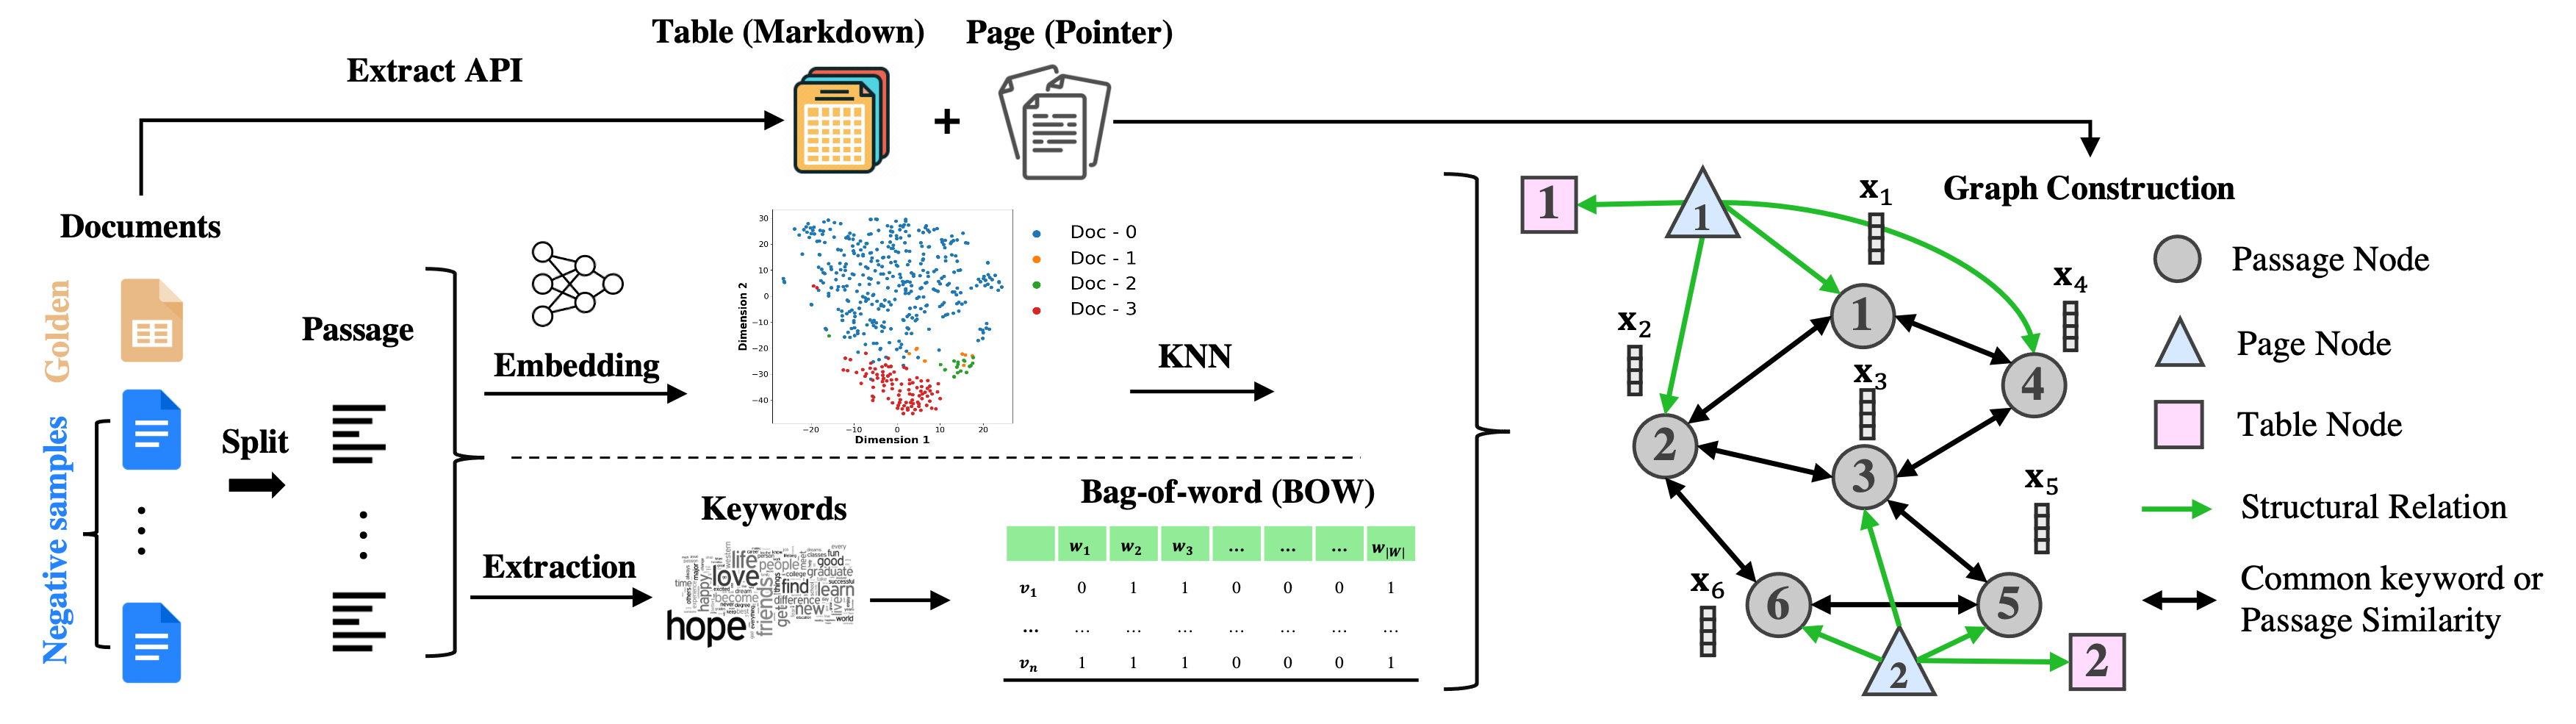
\includegraphics[width=1.0\textwidth]{Figure/graphconstruct.png}
    \caption{Knowledge Graph Construction. We split each document in the document collection into passages. For each passage, we either directly obtain their embeddings via pre-trained encoders or extract their keywords to build bag-of-word (BOW) features. Then we connect two passages based on their embedding similarity or whether they share common keywords. Additionally, we extract tables/pages via Extract-PDF API and add them as structural nodes to the KG. If pages include passages and tables, we add a directed edge to denote the belonging relations. The table nodes include the markdown formatted content of that table as Figure~\ref{fig-tableunderstanding} in Supplementary has empirically shown that LLMs are able to understand tables in this format.}
    \label{fig-graphconstruct}
    \vspace{-2ex}
\end{figure*}

Following~\cite{tian2023heterogeneous}, let $G = (\mathcal{V}, \mathcal{E})$ be a knowledge graph constructed from a set of documents $\mathcal{D}$, where the node set $\mathcal{V}=\{v_i\}_{i = 1}^{n}$ representing document structures (e.g., passages/pages/tables, etc.) and the edge set $\mathcal{E}\subset \mathcal{V}\times \mathcal{V}$ representing the connections among different nodes (e.g., semantic/lexical similarity and belonging relations among document structures, etc.). Let $\mathcal{X} = \{\mathcal{X}_i\}_i^{n}$ be node features and $\mathcal{X}_i$ corresponds to the feature of node $v_i$, the form of which could be the text for the passage, the markdown for the table and the page number for the page.

% For each node, $v_i$ and edge $e_{ij}$, their type mapping functions are $\tau(v_{i}): \mathcal{V} \rightarrow \mathcal{A}$ and $\phi(e_{ij}): \mathcal{E} \rightarrow \mathcal{R}$, respectively. 

% Additionally, we collect sequential data for fine-tuning our graph traverser. Let $\mathcal{S} = \{\mathcal{S}^m\}_{m = 1}^{M}$ be the observed sentence sequences with $m^{\text{th}}$ sequence as $\mathcal{S}^m = \{s_i^m\}_{i = 0}^{|\mathcal{S}^m|}$, which starts with a question and sequentially traverse among supporting facts to establish the grounding contexts for answering the question. The details of collecting the sequential data $\mathcal{S}$ are discussed in Supplementary~\ref{sup-datacollect}.

% Next, we introduce how we construct the knowledge graph given a collection of documents.